% want your title page.
% OR
% 2) Remove everything outside the \begin{titlepage} and \end{titlepage} and 
% move this file to the same directory as the LaTeX file you wish to add it to. 
% Then add \input{./title_page_1.tex} to your LaTeX file where you want your
% title page.
%
%%%%%%%%%%%%%%%%%%%%%%%%%%%%%%%%%%%%%%%%%
%\title{Title page with logo}
%----------------------------------------------------------------------------------------
%	PACKAGES AND OTHER DOCUMENT CONFIGURATIONS
%----------------------------------------------------------------------------------------

\documentclass[12pt]{article}
\usepackage[english]{babel}
\usepackage[utf8x]{inputenc}
\usepackage{amsmath}
\usepackage{graphicx}
\usepackage[colorinlistoftodos]{todonotes}
\usepackage{listings}
\usepackage{caption}
\usepackage{parskip} %dannati indent


\captionsetup[lstlisting]{singlelinecheck=false, margin=0pt, font={bf,footnotesize} }
\renewcommand\lstlistingname{}
\lstset{escapeinside={<@}{@>}}
\definecolor{comment}{RGB}{237, 141, 33}
\definecolor{backy}{RGB}{ 255, 253, 183 }
\definecolor{back}{RGB}{ 30,30,30 }
\definecolor{shadecolor}{RGB}{ 30,30,30 }
\definecolor{purple}{RGB}{155, 40, 140}
\lstset{
%rulecolor=\color{white},
numbers=left,
numberstyle=\color{black},
%backgroundcolor=\color{back},   
frame=single,
showspaces=false,
basicstyle=\ttfamily,%\color{white},
showstringspaces=false,
keywordstyle=\color{purple},       % keyword style
commentstyle=\color{comment},    % comment style
stringstyle=\color{blue}    % string literal style
}

\lstdefinestyle{ANTLR}{
    basicstyle=\fontsize{9}{11}\ttfamily\color{black},%
    breaklines=true,%                                      allow line breaks
    moredelim=[s][\color{green!50!black}\ttfamily]{'}{'},% single quotes in green
    moredelim=*[s][\color{black}\ttfamily]{options}{\}},%  options in black (until trailing })
    commentstyle={\color{gray}\itshape},%                  gray italics for comments
    morecomment=[l]{//},%                                  define // comment
    emph=[1]{%
    TWODOT,CMP,DTYPE,VTYPE,RTYPE,JMP,ADDI,SUBI,ANDI,ORI,XORI,ADD,SUB,MUL,XOR,OR,AND,INT,WS,STRING,ERROR%                                      literal strings listed here
        },emphstyle=[1]{\color{blue}\ttfamily},%              and formatted in blue
    emph=[2]{start,line,defineVar,reserveVar,defineRegister,r3IType,r3Type,f3,fI,register,immediateVar,jumpCond,condition,jumpUnc,label
        },emphstyle=[2]{\color{purple}\ttfamily},
    alsoletter={:,|,;},%
    morekeywords={:,|,;},%                                 define the special characters
    keywordstyle={\color{black}},%                         and format them in black
}




\begin{document}

\begin{titlepage}

\newcommand{\HRule}{\rule{\linewidth}{0.5mm}} % Defines a new command for the horizontal lines, change thickness here

\center % Center everything on the page
 
%----------------------------------------------------------------------------------------
%	HEADING SECTIONS
%----------------------------------------------------------------------------------------

\textsc{\LARGE Università di Bergamo}\\[1.5cm] % Name of your university/college
\textsc{\Large Relazione progetto}\\[0.5cm] % Major heading such as course name
\textsc{\large Linguaggi Formali e Compilatori}\\[0.5cm] % Minor heading such as course title

%----------------------------------------------------------------------------------------
%	TITLE SECTION
%----------------------------------------------------------------------------------------

\HRule \\[0.4cm]
{ \huge \bfseries Parser ISA Risc-V}\\[0.4cm] % Title of your document
\HRule \\[1.5cm]
 
%----------------------------------------------------------------------------------------
%	AUTHOR SECTION
%----------------------------------------------------------------------------------------

\begin{minipage}{0.4\textwidth}
\begin{flushleft} \large
\emph{Autore:}\\
Dario \textsc{Sardi} % Your name
\end{flushleft}
\end{minipage}
~
\begin{minipage}{0.4\textwidth}
\begin{flushright} \large
\emph{Supervisore:} \\
Giuseppe \textsc{Psaila} % Supervisor's Name
\end{flushright}
\end{minipage}\\[2cm]

% If you don't want a supervisor, uncomment the two lines below and remove the section above
%\Large \emph{Author:}\\
%John \textsc{Smith}\\[3cm] % Your name

%----------------------------------------------------------------------------------------
%	DATE SECTION
%----------------------------------------------------------------------------------------

{\large 12 Marzo 2019}\\[2cm] % Date, change the \today to a set date if you want to be precise

%----------------------------------------------------------------------------------------
%	LOGO SECTION
%----------------------------------------------------------------------------------------


\includegraphics[scale=0.5]{logo.png}\\[1cm] % Include a department/university logo - this will require the graphicx package
 
%----------------------------------------------------------------------------------------

\vfill % Fill the rest of the page with whitespace

\end{titlepage}


\begin{abstract}
Il progetto è volto allo sviluppo di un traduttore di un subset di istruzioni appartenenti all'ISA RISC-V da linguaggio assembly a linguaggio naturale.
\end{abstract}
\section{Output e Input}
Il programma prende come input il testo contenuto nel file "resources/input.file" e restituisce la traduzione in linguaggio naturale come output su terminale seguito da una eventuale lista di errori.
\\Un esempio di output privo di errori:
\begin{lstlisting}
    <@\textcolor{purple}{----- PARSING STARTED-------}@>
created ADDI between 1 and 12 to be saved at 10
created OR between 12 and 2 to be saved at 5
added label li
created ADD between 7 and 5 to be saved at 22
created AND between 7 and 5 to be saved at 23
jump to li at line 3 if condition is true
created OR between 22 and 23 to be saved at 24
<@\textcolor{purple}{----- PARSING DONE -------}@>
\end{lstlisting}
In caso di errori l'output è il seguente:
\begin{lstlisting}
    <@\textcolor{purple}{----- PARSING STARTED-------}@>
created ADDI between 1 and 12 to be saved at 10
created OR between 12 and 2 to be saved at 5
added label li
created ADD between 7 and 5 to be saved at 22
created AND between 7 and 45 to be saved at 23

#############################
#  ERROR! PARSING STOPPED!  #
#############################
<@\textcolor{red}{ERRORS:}@>
1. label 'li' at line 4 already exist, ignoring it.
2. Lexer error at [6:15].Max register value is 30!
\end{lstlisting}






%%%%%%%%%%%%%%%%%%%%%%%%%%%%%%%%%%%%%%%%%%%%%%%%%%%%%%%%%%%%%%%%%%%%%
\section{Registri e immediati}
Le specifiche scelte per questo progetto prevedono 30 registri indirizzabili attraverso la sequenza '0xNumeroDiRegistro' dove il numero del registro è un numero intero compreso fra 0 e 30.
\\La scelta del prefisso è stata dettata dalla necessità di distinguere numeri interi e numeri dei registri durante il parsing e rendere il meno confusionario possibile il codice.
\\Per quanto riguarda gli immediati è stata prevista la dimensione massima di una word su ISA RISC-V equivalente al valore decimale 4096.
%%%%%%%%%%%%%%%%%%%%%%%%%%%%%%%%%%%%%%%%%%%%%%%%%%%%%%%%%%%%%%%%%%%%%
\section{Variabili}
È previsto l'utilizzo di variabili statiche per etichettare registri o valori notevoli.
La sintassi per dichiarare il nome di un registro è:
\begin{lstlisting}[numbers=none]
    <@\textcolor{purple}{DR}@> <@\textcolor{orange}{etichetta}@> <@\textcolor{blue}{0xNumeroDiRegistro}@>
\end{lstlisting}
Una definizione valida può essere dunque:
\begin{lstlisting}[numbers=none]
    <@\textcolor{purple}{DR}@> <@\textcolor{orange}{RegistroA}@> <@\textcolor{blue}{0x9}@>
\end{lstlisting}
Si ricorda che il valore massimo assegnabile ad un registro è pari a 0x30 per specifiche precedentemente definite.
Per quanto riguarda le variabili, si possono creare variabili numeriche statiche di tipo Byte e Word.
Risulta possibile riservare una variabile senza inizializzarla attraverso il comando RESB per riservare un Byte  e RESW per riservare una Word.
\\Esempio di variabili riservate sono:
\begin{lstlisting}[numbers=none]
    <@\textcolor{purple}{RESW}@> <@\textcolor{orange}{valoreMassimo}@>
    <@\textcolor{purple}{RESB}@> <@\textcolor{orange}{threshold}@>
\end{lstlisting}
Questa operazione è stata introdotta per una implementazione futura dove variabili dinamiche potranno essere assegnate o variate utilizzandole come destinazione all'interno di funzioni.
Il comando attualmente utile risulta essere la dichiarazione di una variabile con relativa inizializzazione effettuabile tramite:
\begin{lstlisting}[numbers=none]
    <@\textcolor{purple}{DW}@> <@\textcolor{orange}{valoreMassimo}@> <@\textcolor{blue}{3623}@>
    <@\textcolor{purple}{DB}@> <@\textcolor{orange}{threshold}@> <@\textcolor{blue}{90}@>
\end{lstlisting}


\subsection{Error handling}
Nel caso di una dichiarazione di variabile troppo grande il programma risponderà settando la variabile a 0 e proseguendo normalmente.
\\Esempi di input-output possibili sono:
\begin{lstlisting}[caption=input]
    <@\textcolor{purple}{DW}@> <@\textcolor{orange}{ciao}@> <@\textcolor{blue}{5400}@>
\end{lstlisting}
\begin{lstlisting}[caption=output]
   <@\textcolor{purple}{----- PARSING STARTED-------}@>
    defined new Word-type variable with value 0 
    named <@\textcolor{orange}{ciao}@>
   <@\textcolor{purple}{----- PARSING DONE -------}@>
   <@\textcolor{red}{ERRORS:}@>
   1.	variable value is not Word type
        (max value 4096), <@\textcolor{orange}{ciao}@> set to 0
\end{lstlisting}
Oppure:
\begin{lstlisting}[caption=input]
    <@\textcolor{purple}{DB}@> <@\textcolor{orange}{ciao}@> <@\textcolor{blue}{300}@>
\end{lstlisting}
\begin{lstlisting}[caption=output]
   <@\textcolor{purple}{----- PARSING STARTED-------}@>
    defined new Byte-type variable with value 0 
    named <@\textcolor{orange}{ciao}@>
   <@\textcolor{purple}{----- PARSING DONE -------}@>
   <@\textcolor{red}{ERRORS:}@>
   1.	variable value is not Byte type
        (max value 256), <@\textcolor{orange}{ciao}@> set to 0
\end{lstlisting}
\newpage
Altro errore può verificarsi nella dichiarazione di un registro dal numero superiore al 30 come ad esempio:

\begin{lstlisting}[caption=input]
    <@\textcolor{purple}{DR}@> <@\textcolor{orange}{reg1}@> <@\textcolor{blue}{0x50}@>
\end{lstlisting}

\begin{lstlisting}[caption=output]
    <@\textcolor{purple}{----- PARSING STARTED-------}@>
    variable <@\textcolor{orange}{reg}@> too big for register-type, set to 0
    <@\textcolor{purple}{----- PARSING DONE -------}@>
    <@\textcolor{red}{ERRORS:}@>
    1.	Lexer error at [1:9].Max register 
        value is 30!
\end{lstlisting}

Nel caso di un assegnamento ad una variabile registro un valore immediato, l'errore viene considerato grave e il parsing interrotto.



%%%%%%%%%%%%%%%%%%%%%%%%%%%%%%%%%%%%%%%%%%%%%%%%%%%%%%%%%%%%%%%%%%%%%
\newpage
\section{Le funzioni}
Il subset di istruzioni considerato prevede due tipologie di funzioni, le R-type e le I-type.
\begin{figure}[h]
    \centering
    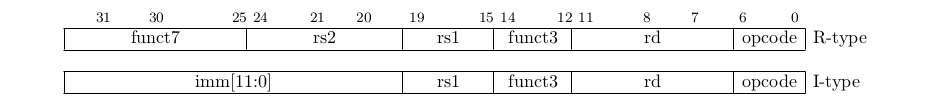
\includegraphics[scale=0.5]{functionTypes.png}
    \caption{Struttura in binario delle funzioni e relativi attributi}
    \label{fig:err1}
\end{figure}
\\
In entrambe le funzioni la struttura sintattica risulta essere
\begin{lstlisting}[numbers=none]
    <@\textcolor{purple}{Funzione}@> <@\textcolor{blue}{Destinazione Operando1 Operando2}@>
\end{lstlisting}
Per le funzioni R-type destinazione e operandi saranno registri
\begin{lstlisting}[numbers=none]
    <@\textcolor{purple}{Funzione}@> <@\textcolor{blue}{RegDestinazione RegOperando1 RegOperando2}@>
\end{lstlisting}
Per le funzioni di I-type il secondo operando dovrà essere un immediato
\begin{lstlisting}[numbers=none]
    <@\textcolor{purple}{Funzione}@> <@\textcolor{blue}{RegDestinazione RegOperando1}@> <@\textcolor{orange}{ImmOperando2}@>
\end{lstlisting}

Le funzioni previste sono le seguenti: 
\begin{enumerate}
    \item \textcolor{purple}{R-Type: ADD,SUB,MUL,OR,XOR,AND}
    \item \textcolor{purple}{I-Type: ADDI,SUBI,ORI,XORI,ANDI}
\end{enumerate}
Esempi di funzioni sono :
\begin{lstlisting}[caption=input]
    <@\textcolor{purple}{ADDI}@> <@\textcolor{blue}{0x10 0x01}@> <@\textcolor{orange}{12}@>
    <@\textcolor{purple}{OR}@> <@\textcolor{blue}{0x05 0x12 0x02}@>
\end{lstlisting}
\begin{lstlisting}[caption=output]
    <@\textcolor{purple}{ ----- PARSING STARTED------- }@>
    created ADDI between 1 and 12 to be saved at 10
    created OR between 12 and 2 to be saved at 5
    <@\textcolor{purple}{ ----- PARSING DONE------- }@>
\end{lstlisting}
\subsection{Error Handling}
Gli unici errori possibili in una funzione sono l'utilizzo di numeri di registri errati,di variabili errate (registro al posto di immediato e viceversa) o immediati di dimensione superiore alla word.
\\Nel caso di registri troppo grandi l'errore è trasmesso direttamente dal controllo su ogni singolo valore di registro e causa l'interruzione del parsing.
\begin{lstlisting}[caption=input]
    <@\textcolor{purple}{DR}@> <@\textcolor{orange}{reg}@> <@\textcolor{blue}{0x10}@>
    <@\textcolor{purple}{ADD}@> <@\textcolor{orange}{reg reg}@> <@\textcolor{blue}{0x50}@> 
\end{lstlisting}

\begin{lstlisting}[caption=output]
    <@\textcolor{purple}{ ----- PARSING STARTED------- }@>
    defined new Register variable with value 
     10 named <@\textcolor{orange}{reg}@> 

    #############################
    #  ERROR! PARSING STOPPED!  #
    #############################
    <@\textcolor{red}{ERRORS:}@>
    1.	Lexer error at [2:14].Max register value 
        is 30!
\end{lstlisting}
\newpage
L'utilizzo di variabili errate è contemplato e causa l'interruzione del parsing:
\begin{lstlisting}[caption=input]
    <@\textcolor{purple}{DR}@> <@\textcolor{orange}{reg}@> <@\textcolor{blue}{0x10}@>
    <@\textcolor{purple}{DW}@> <@\textcolor{orange}{c}@> <@\textcolor{blue}{12}@>
    <@\textcolor{purple}{ADD}@> <@\textcolor{orange}{reg reg c}@> 
\end{lstlisting}
\begin{lstlisting}[caption=output]
    <@\textcolor{purple}{ ----- PARSING STARTED------- }@>
    defined new Register variable with value 
     10 named <@\textcolor{orange}{reg}@> 
    defined new Word-type variable with value 
     12 named <@\textcolor{orange}{c}@>
    
    #############################
    #  ERROR! PARSING STOPPED!  #
    #############################
    <@\textcolor{red}{ERRORS:}@>
    1.	at line 3 using a non register variable
\end{lstlisting}

\newpage
%%%%%%%%%%%%%%%%%%%%%%%%%%%%%%%%%%%%%%%%%%%%%%%%%%%%%%%%%%%%%%%%%%%%%
\section{Jump}
Sono state implementate chiamate di salto condizionate e non, non prevedendo chiamate a label non ancora definiti (jump ahead).
Le jump consistono in un label definito come una stringa seguita da due punti e una chiamata di salto al label stesso.
\\Chiamate incondizionate si effettuano tramite "JMP" seguito dal label desiderato:
\begin{lstlisting}[caption=input]
    <@\textcolor{orange}{jumplabel}@> :
    DR reg 0x10
    ADD reg reg 0x20
    JMP <@\textcolor{orange}{jumplabel}@>
\end{lstlisting}

\begin{lstlisting}[caption=output]
    <@\textcolor{purple}{ ----- PARSING STARTED------- }@>
    added label <@\textcolor{orange}{jumplabel}@>
    defined new Register variable with value 10 
     named reg
    created ADD between 10 and 20 to be saved at 10
    jump to <@\textcolor{orange}{jumplabel}@> at line 1
    <@\textcolor{purple}{----- PARSING DONE -------}@>
\end{lstlisting}
Per salti condizionati si ha una comparazione fra valori di registro che nel caso risulti corretta permette il salto.
\\Funzioni di comparazione possono essere:
\begin{enumerate}
    \item JE/JZ     Jump Equal or Jump Zero
    \item JNE/JNZ 	Jump not Equal or Jump Not Zero
    \item JG/JNLE 	Jump Greater or Jump Not Less/Equal 
    \item JGE 	    Jump Greater/Equal
    \item JL/JNGE 	Jump Less or Jump Not Greater/Equal
    \item JLE/JNG 	Jump Less/Equal or Jump Not Greater
\end{enumerate}
Esempio di salto condizionato:
\begin{lstlisting}[caption=input]
    <@\textcolor{orange}{jumplabel}@> :
    DR reg 0x10
    ADD reg reg 0x20
    CMP 0x10 0x11
    JNE <@\textcolor{orange}{jumplabel}@>
\end{lstlisting}
\begin{lstlisting}[caption=output]
    <@\textcolor{purple}{ ----- PARSING STARTED------- }@>
    added label <@\textcolor{orange}{jumplabel}@>
    defined new Register variable with value 10 
     named reg
    created ADD between 10 and 20 to be saved at 10
    comparing register 10 to 11
    jump to <@\textcolor{orange}{jumplabel}@> at line 1
     if condition is true
    <@\textcolor{purple}{----- PARSING DONE -------}@>
\end{lstlisting}




\newpage
\subsection{Error Handling}
Nel caso di label ripetuti solo il primo viene considerato e i successivi vengono ignorati.
\begin{lstlisting}[caption=input]
    <@\textcolor{orange}{jumplabel}@> :
    DR reg 0x10
    ADD reg reg 0x20
    <@\textcolor{orange}{jumplabel}@> :
    CMP 0x10 0x11
    JNE <@\textcolor{orange}{jumplabel}@>
\end{lstlisting}
\begin{lstlisting}[caption=output]
    <@\textcolor{purple}{ ----- PARSING STARTED------- }@>
    added label <@\textcolor{orange}{jumplabel}@>
    defined new Register variable with value 10 
     named reg
    created ADD between 10 and 20 to be saved at 10
    comparing register 10 to 11
    jump to <@\textcolor{orange}{jumplabel}@> at line 1
     if condition is true
    <@\textcolor{purple}{----- PARSING DONE -------}@>
    <@\textcolor{red}{ERRORS:}@>
    1.	label 'jumplabel' at line 4 already exist, 
        ignoring it.
\end{lstlisting}
\newpage
Nel caso di salti a label non esistenti il programma si interrompe segnalando l'errore.
\begin{lstlisting}[caption=input]
    <@\textcolor{orange}{jumplabel}@> :
    DR reg 0x10
    ADD reg reg 0x20
    CMP 0x10 0x11
    JNE <@\textcolor{orange}{somewhere}@>
\end{lstlisting}
\begin{lstlisting}[caption=output]
    <@\textcolor{purple}{ ----- PARSING STARTED------- }@>
    added label <@\textcolor{orange}{jumplabel}@>
    defined new Register variable with value 10 
     named reg
    created ADD between 10 and 20 to be saved at 10
    comparing register 10 to 11
    
    #############################
    #  ERROR! PARSING STOPPED!  #
    #############################
    <@\textcolor{red}{ERRORS:}@>
    1.	Label <@\textcolor{orange}{somewhere}@> at line 5 does not exist! 
        STOPPING PARSER!
\end{lstlisting}
\newpage
%%%%%%%%%%%%%%%%%%%%%%%%%%%%%%%%%%%%%%%%%%%%%%%%%%%%%%%%%%%%%%%%%%%%%%%%%%%%
\section{ANTLR grammatica}
Variabili dichiarate per il lexer:
\begin{lstlisting}[style=ANTLR,caption=lexer]
    
TWODOT	:	':';
CMP	:	'CMP';
DTYPE	:	'DB'|'DW';
VTYPE	:	'RESB' | 'RESW';
RTYPE	:	'DR'| 'DRR';
JMP	:	'JMP' | 'JE'  | 'JZ' | 
		'JNE' | 'JNZ' | 'JG' | 
		'JNLE'| 'JGE' | 'JNG'| 
		'JL'  |'JNGE' | 'JLE';
ADDI	:	'addi'	| 'ADDI';
SUBI	:	'subi'	| 'SUBI';
ANDI	:	'andi'	| 'ANDI';
ORI	:	'ori'	| 'ORI;';
XORI	:	'xori'  | 'XORI'; 
ADD	:	'add' 	| 'ADD';
SUB	:	'sub' 	| 'SUB';
MUL	:	'mul'	| 'MUL';
XOR	:	'xor'	| 'XOR';
OR	:	'or' 	| 'OR';
AND	:	'and' 	| 'AND';
INT	:    	('0'..'9')+;
WS      :   (
        ' '
        |'\t'
            | '\r'
            )+ {$channel=HIDDEN;}
        ;

STRING	:	('a'..'z'|'A'..'Z')+;
ERROR : . {System.out.println("what?...");} ;
\end{lstlisting}
\newpage
Il parser inizia considerando come istruzioni valide funzioni, dichiarazioni di variabili, label e jump separate dal terminatore di linea.
La grammatica priva delle parti relative a java si presenta cosi: 
\begin{lstlisting}[style=ANTLR,caption=parser]
    
start           : line* ;

line            : (r3Type | r3IType | defineVar | reserveVar | 
                  defineRegister | jumpUnc | jumpCond | label
                  | ERROR ) '\n';

defineVar       : DTYPE STRING INT ;
	
reserveVar      : VTYPE STRING ;
    
defineRegister	: RTYPE STRING register ;

r3IType	        : fI register register ( immediateVar | INT );

r3Type      	: f3 register register register ;

f3              : ADD | SUB | MUL | XOR | OR | AND ;

fI              : ADDI | ANDI | ORI | SUBI | XORI ; 

register        : '0x' INT  | STRING ;
		
immediateVar    : STRING ;

jumpCond        : condition '\n' jumpUnc  ;

condition       : CMP register register ;

jumpUnc         : JMP STRING ;
	
label 	        : STRING TWODOT ;
\end{lstlisting}
%%%%%%%%%%%%%%%%%%%%%%%%%%%%%%%%%%%%%%%%%%%%%%%%%%%%%%%%%%%%%%%%%%%%%
\end{document}